\documentclass{standalone}
\usepackage{tikz}
\usepackage{xinttools}

\usetikzlibrary{calc,math}



\begin{document}

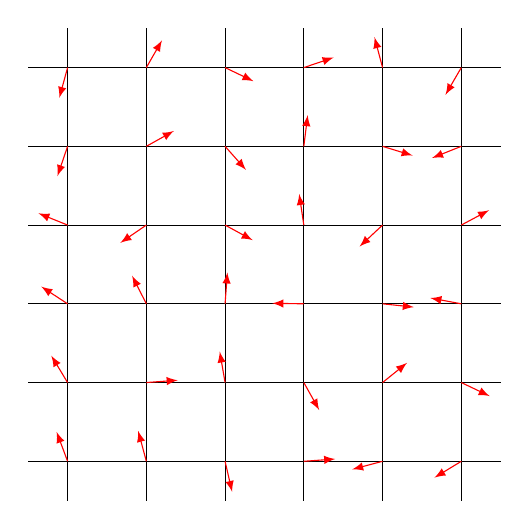
\begin{tikzpicture}
  \draw (-0.5,-0.5) grid (5.5, 5.5);

  \foreach \x in {0,...,5} {
    \foreach \y in {0,...,5} {
      \tikzmath{
        real \a;
        \a = random() * 360;
      }
      \draw[-latex,red] (\x, \y) -- ++(\a:0.4);
    }
  }
\end{tikzpicture}

\end{document}
